\documentclass{beamer}
\mode<presentation>

\usepackage{pgfpages}
\usepackage{bbm}
\usepackage{amsmath}
\usepackage{amssymb} 
\usepackage{amsthm}
\usepackage{epsfig}
\usepackage{graphicx}
\usepackage{natbib}

\graphicspath{{./figures/}}

\makeatletter 
\def\newblock{\beamer@newblock} 
\makeatother  

% set color and font of frametitles
\setbeamercolor{frametitle}{fg=blue}
%\setbeamerfont{frametitle}{series=\bfseries}

\newcommand{\red}[1]{{\color{red} #1}}
\newcommand{\blue}[1]{{\color{blue} #1}}
\newcommand{\avg}[1]{\left\langle #1 \right\rangle}

\newcommand{\code}[1]{{\fontfamily{pcr}\selectfont \textbf{#1}}}

%%%%%%%%%%%%%%%%%%%%%%%%%%%%%%%%%%%%%%%%%%%%%%%%%%%%%%%%%%%%%%%%%
%% SETTINGS

% set item type and color
\setbeamercolor{item}{fg=black}  % set color
\setbeamertemplate{itemize items}[circle] % if you want a circle
\setbeamertemplate{itemize subitem}[ball] % if you wnat a ball
\setbeamertemplate{itemize subsubitem}[triangle] % if you want a triangle

% set spacing for itemize
\setbeamertemplate{itemize/enumerate subbody begin}{\vspace{0.1cm}}
\setbeamertemplate{itemize/enumerate subbody end}{\vspace{0.1cm}}

%% END SETTINGS
%%%%%%%%%%%%%%%%%%%%%%%%%%%%%%%%%%%%%%%%%%%%%%%%%%%%%%%%%%%%%%%%%%%

% remove navigation symbols
\beamertemplatenavigationsymbolsempty 

\title{Version control management and research collaboration using git and github}
\subtitle{An introduction}
\author{APSIS group}
\institute{MCC Berlin}
\date{July 11th, 2019}
\titlegraphic{
\includegraphics[width=3cm]{images/Git-logo.png}\hspace*{1cm}~%
   
\includegraphics[width=1.5cm]{images/github-logo.png}
}

\AtBeginSection[]
  {
     \begin{frame}<beamer>
     \frametitle{}
     \tableofcontents[currentsection]
     \end{frame}
  }

\begin{document}

\maketitle


\section{What is git and GitHub and why to use them?}

% ==============================================================
\begin{frame}
\frametitle{What is version control?}


\begin{columns}
	\begin{column}{0.75\linewidth}

A software (component) to keep track of the history of revisions and/or different versions of files, e.g. documents or programs

\bigskip

Revision are associated with a person and timestamp

\bigskip

Dependencies between versions as a graph

\bigskip

Version control system: standalone software to record changes to files

\bigskip

Most used systems: git, Apache Subversion (SVN), CVS, other commercial systems

	\end{column}
		\begin{column}{0.25\linewidth}
		\begin{figure}
			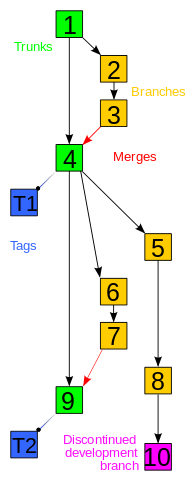
\includegraphics[width=\linewidth]{images/Revision_controlled_project_visualization.png}
			Source: wikipedia.org
		\end{figure}
	\end{column}
\end{columns}

\end{frame}
%--------------------------------------------------------------


% ==============================================================
\begin{frame}
\frametitle{What is git?}

\bigskip

An open source version control system designed for distributed software development

\bigskip

Created in 2005 by Linus Torvalds for his work on the Linux kernel

\bigskip

Repository: directory managed with git, contains the entire version history in hidden .git folder

\vspace{1cm}

		\begin{figure}
			
\includegraphics[width=0.3\linewidth]{images/Git-logo.png}
		\end{figure}

\end{frame}

%--------------------------------------------------------------

\begin{frame}
\frametitle{What is GitHub?}

\bigskip

Hosting provider of public and private remote repositories

\bigskip

Remote repository: shared, central repository that collaborators can compare their local repositories to

\bigskip

Provides also functionality for documentation (wiki) and bug reporting and tracking

\bigskip

Alternative providers: GitLab, BitBucket, SourceForge, Launchpad, etc.


\begin{figure}
	
\includegraphics[width=0.2\linewidth]{images/github-logo.png}
\end{figure}

\end{frame}

%--------------------------------------------------------------


\begin{frame}
\frametitle{Why use version control in research?}


Get some order in the mess of projects by routinely keeping track of changes in
\begin{itemize}
\item data
\item software code/scripts
\item manuscripts for papers
\end{itemize}

\bigskip

Share and publish code, data and documents

\bigskip

Make collaboration easier and attribution of work transparent


\end{frame}
%--------------------------------------------------------------

\begin{frame}
\frametitle{Example 1: https://github.com/mcc-apsis/git-intro}

\begin{figure}
	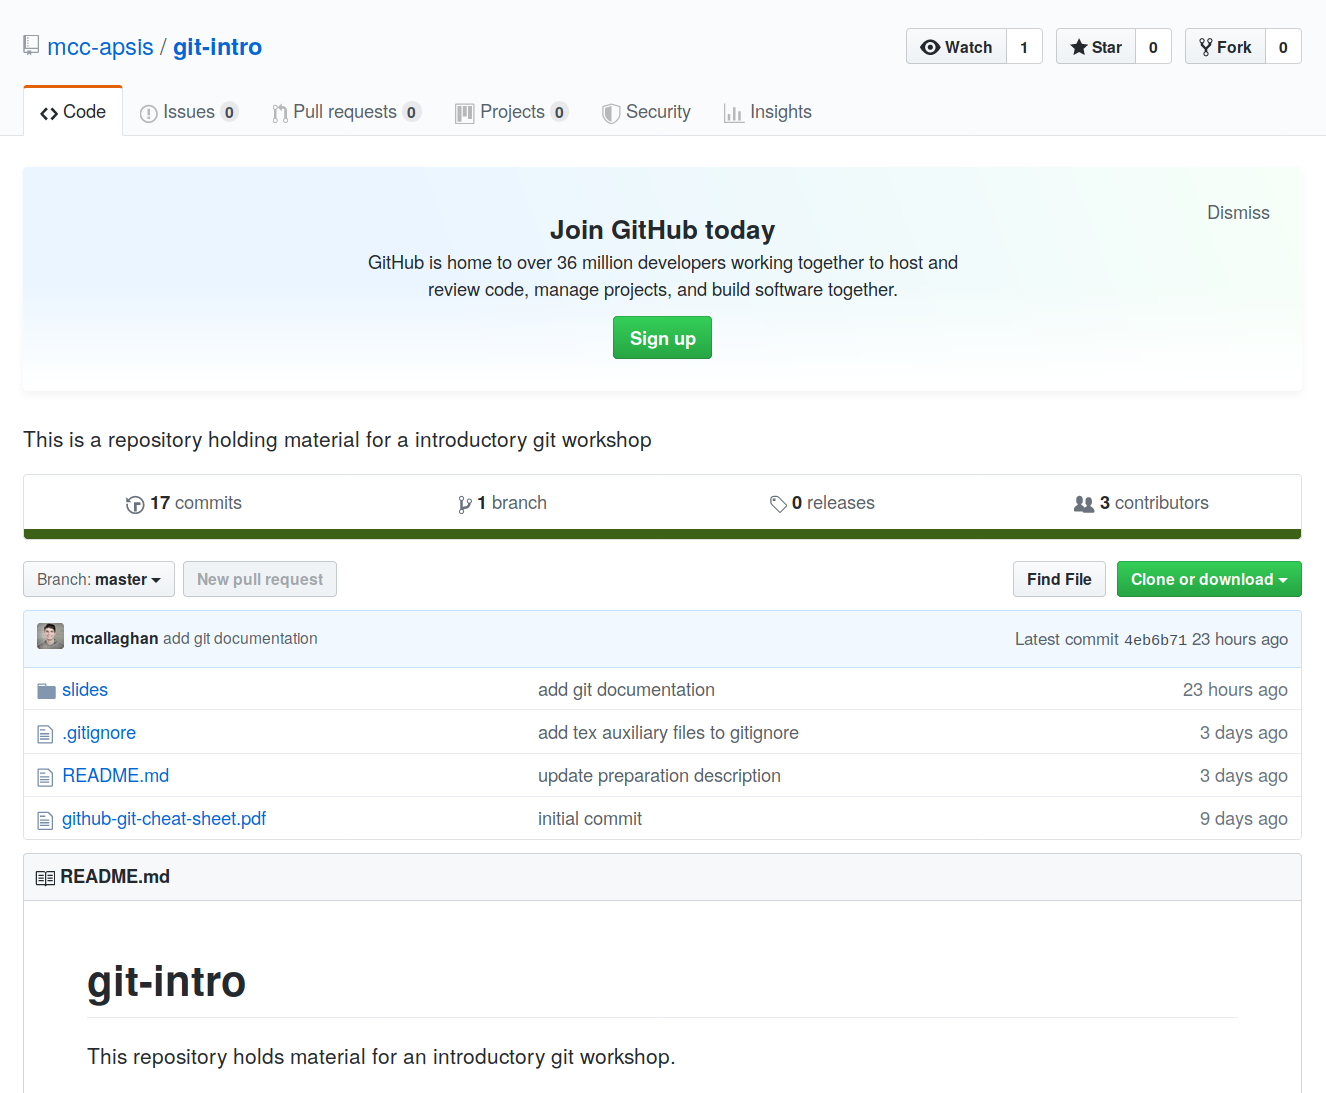
\includegraphics[width=0.95\linewidth]{images/git-intro.png}
\end{figure}


\end{frame}
%--------------------------------------------------------------


\begin{frame}
\frametitle{Example 2: https://github.com/mcc-apsis/plpr-scraper/}

\begin{figure}
	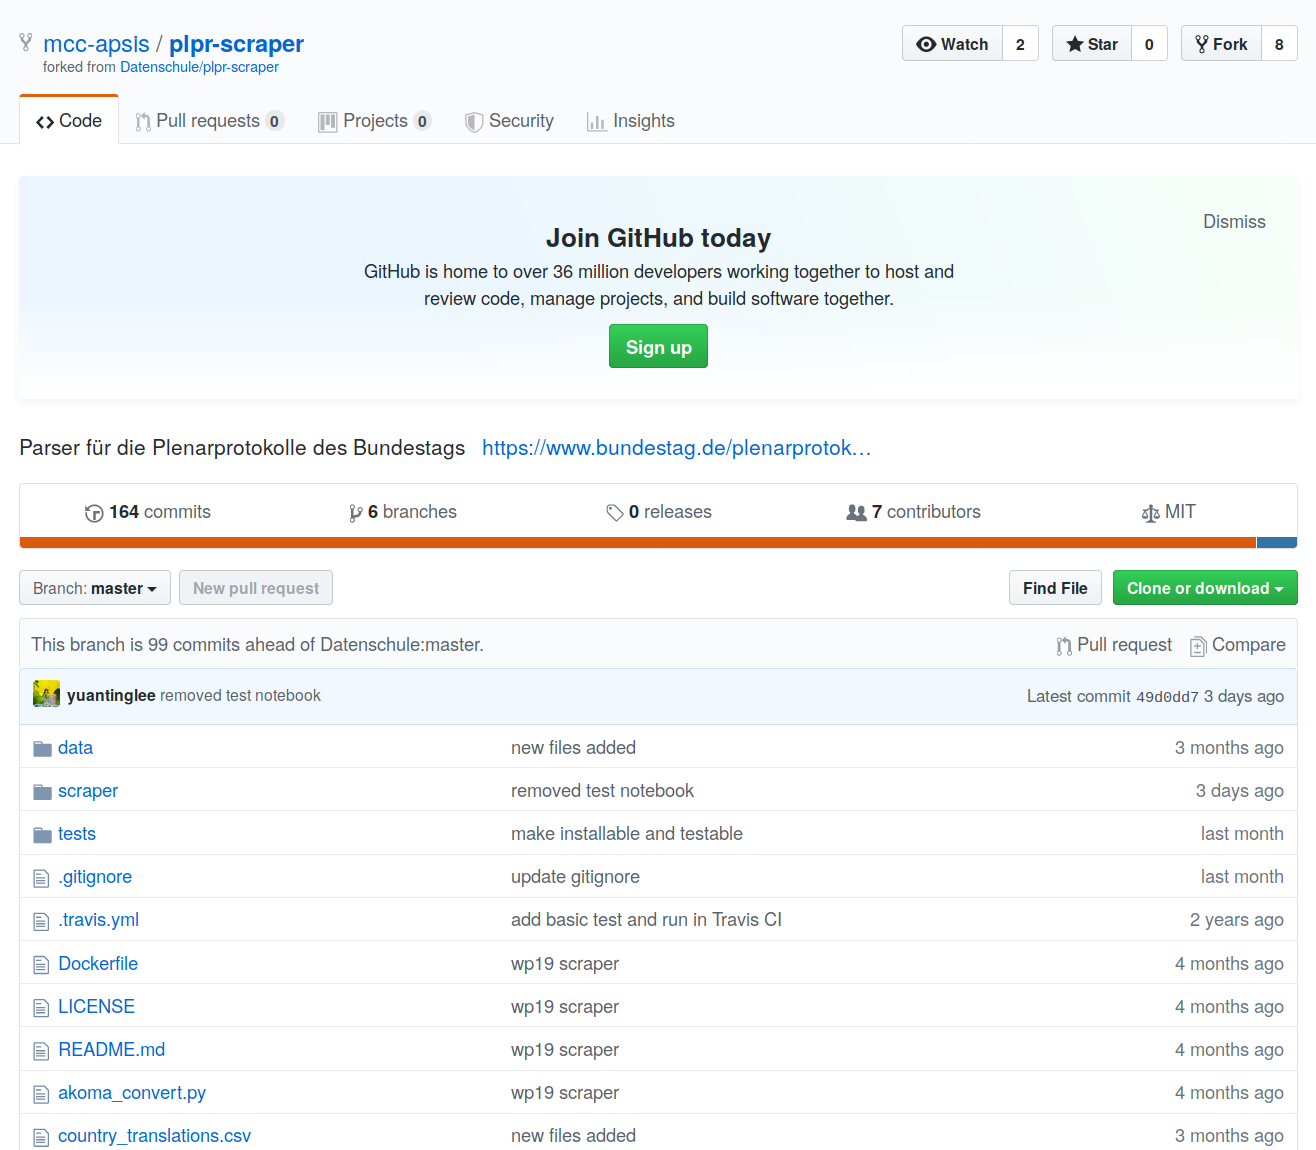
\includegraphics[width=0.95\linewidth]{images/plpr-scraper1.png}
\end{figure}

\end{frame}

%--------------------------------------------------------------

\begin{frame}
\frametitle{Example 2: https://github.com/mcc-apsis/plpr-scraper/}

\begin{figure}
	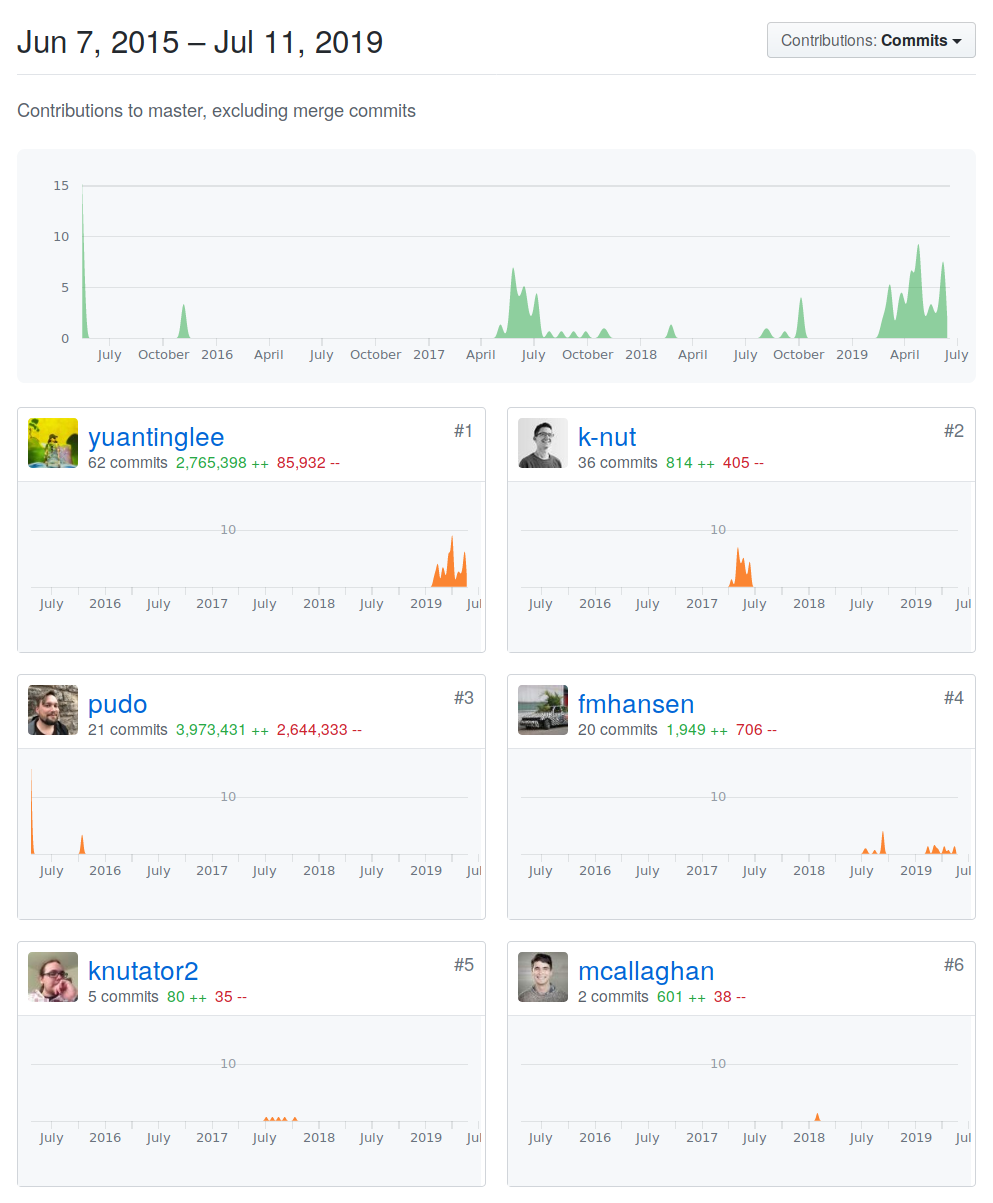
\includegraphics[width=0.75\linewidth]{images/plpr-scraper3.png}
\end{figure}

\end{frame}
%--------------------------------------------------------------

\begin{frame}
\frametitle{Example 2: https://github.com/mcc-apsis/plpr-scraper/}

\begin{figure}
	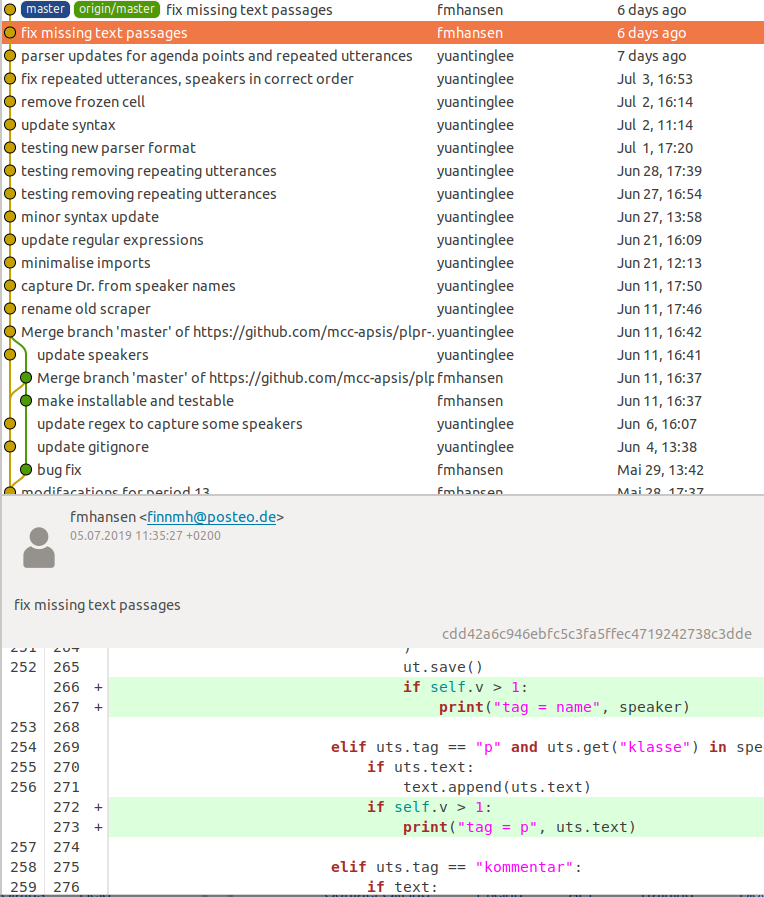
\includegraphics[width=0.8\linewidth]{images/plpr-scraper4.png}
\end{figure}

\end{frame}
%--------------------------------------------------------------

\section{How can I use git and GitHub?}

% ==============================================================
\begin{frame}
\frametitle{Git Workflow (simplest)}

\begin{columns}
	\begin{column}{0.618\linewidth}
		\begin{figure}
			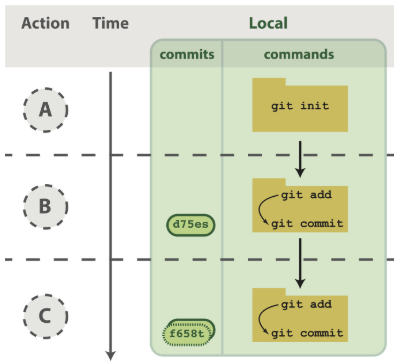
\includegraphics[width=\linewidth]{images/local-workflow}
			\caption{ \cite{Blischak2016}}
		\end{figure}
	\end{column}
	\begin{column}{0.382\linewidth}
		\begin{itemize}
			\item<1-> Keep track of changes in a folder on your computer
			\item<2-> Changes are stored as lines added and removed
			\item<3-> No need to save multiple versions of the same file; you have recorded all changes and can view or revert these at any time
		\end{itemize}
	\end{column}
\end{columns}


\end{frame}
%--------------------------------------------------------------

% ==============================================================
\begin{frame}
\frametitle{Git + Github Workflow (simplest)}

\begin{columns}
	\begin{column}{0.55\linewidth}
		\begin{figure}
			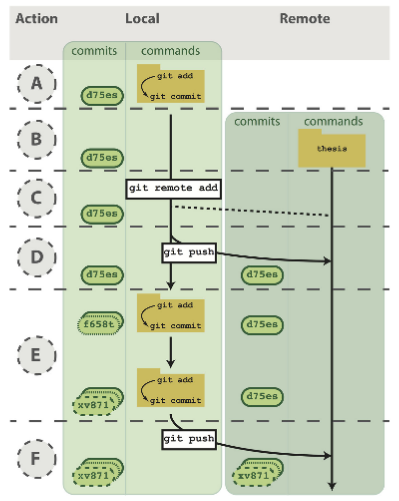
\includegraphics[width=\linewidth]{images/remote-workflow}
		\end{figure}
	\end{column}
	\begin{column}{0.45\linewidth}
		\begin{itemize}
			\item<1-> Attach your repository to a remote version
			\item<2-> If working with collaborators, they also can make a copy (\code{clone}) on their machine
			\item<3-> By both using \code{pull}, you can keep up to date with each others' changes
			\item<4-> For more complicated workflows, especially where maintaining a working version is critical, check out branching \url{https://guides.github.com/introduction/flow/}
		\end{itemize}
	\end{column}
\end{columns}


\end{frame}
%--------------------------------------------------------------



% ==============================================================
\begin{frame}
\frametitle{Tools}

\begin{columns}[t]
	\begin{column}{0.5\linewidth}
		\textbf{Command Line}
		\begin{itemize}
			\item Easy to document/explain
			
			\begin{figure}
				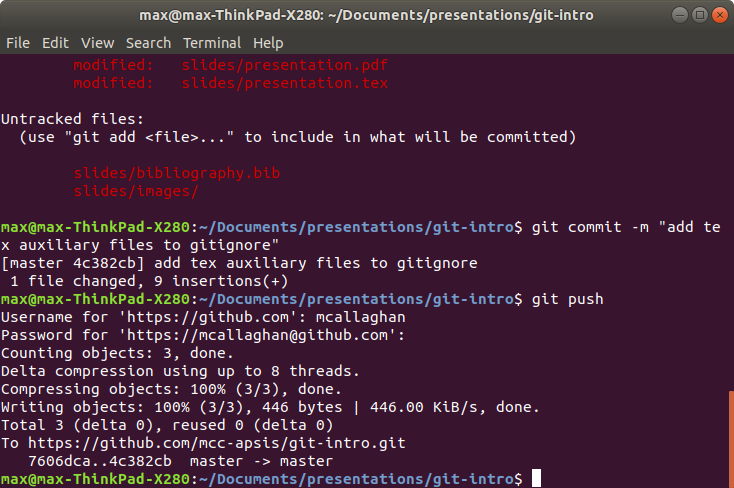
\includegraphics[width=\linewidth]{images/git-terminal}
			\end{figure}
			
			Steeper learning curve, but more flexible and harder to do things unintentionally
		\end{itemize}
	\end{column}

	\begin{column}{0.5\linewidth}
		\textbf{GUIs}
		\begin{itemize}
			\item Easy to use
			
			\begin{figure}
				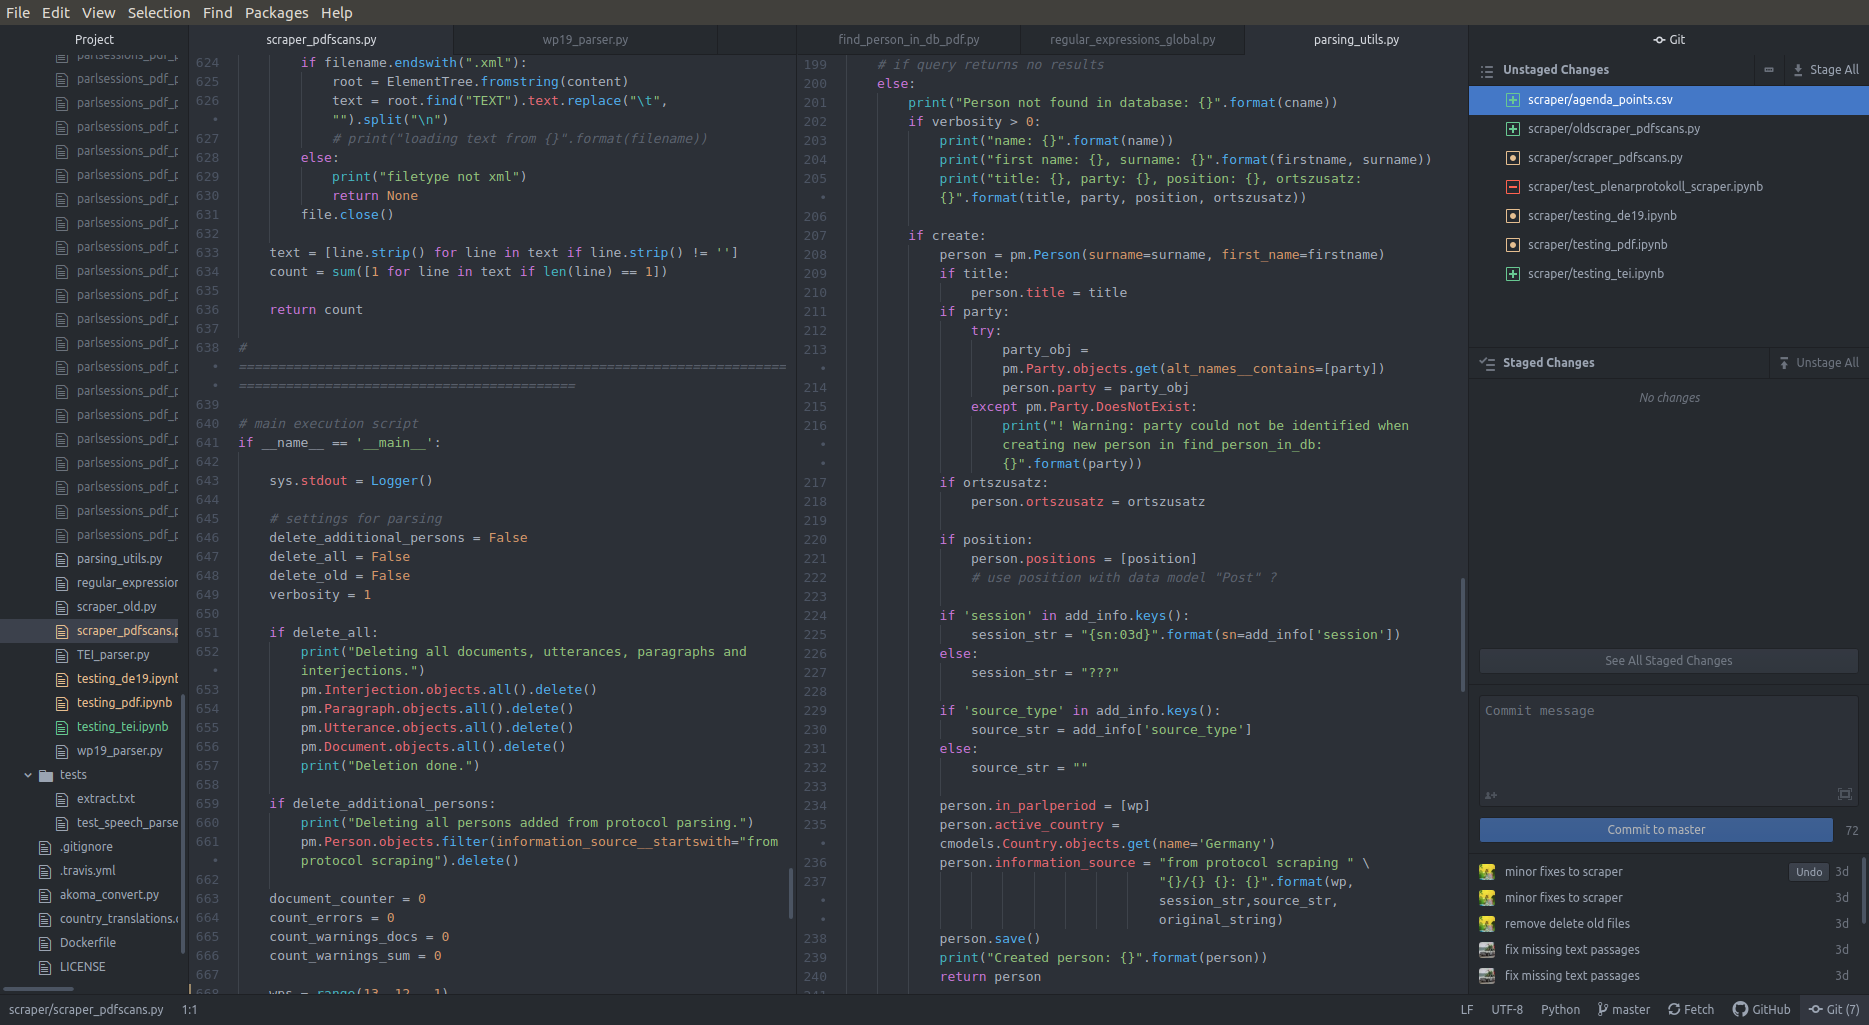
\includegraphics[width=\linewidth]{images/atom-git}
			\end{figure}
			
			Often there are integrations in development environments, e.g. RStudio, Atom
		\end{itemize}
	\end{column}
\end{columns}



\end{frame}
%--------------------------------------------------------------


% ==============================================================
\begin{frame}
\frametitle{Starting a repository}

To start working with a repository, either turn an existing folder into a git repository

\medskip

\code{git init}

\medskip

or copy an existing remote repository into a folder on your machine

\medskip

\code{git clone}

\end{frame}
%--------------------------------------------------------------

% ==============================================================
\begin{frame}
	\frametitle{Editing a respository}
	
	\begin{itemize}
		\item<1-> Edit files (write some new code or a nice new paragraph)
		
\par\noindent\hrulefill\par
		
		\item<2-> Stage changes (tell git about the changes you want record)
		
		\begin{itemize}
			\item \code{git add -A}
			\item Or add only certain files using patterns or exact file names
		\end{itemize}
		
		\par\noindent\hrulefill\par
		
		\item<3-> Commit changes (make a timestamped version of the repository, recording all the changes you have told git about)
		\begin{itemize}
			\item \code{git commit -m ``made a cool new graph''}
			\item It's best if each commit describes a discrete change, and has an interpretable name.
		\end{itemize}
		
		\par\noindent\hrulefill\par
	\end{itemize}
	
	
\end{frame}
%--------------------------------------------------------------

% ==============================================================
\begin{frame}
\frametitle{Managing the repository}

\textbf{Where are we?}

\medskip

\code{git status} tells us which files have changed and are staged or unstaged:

\only{\begin{figure}
	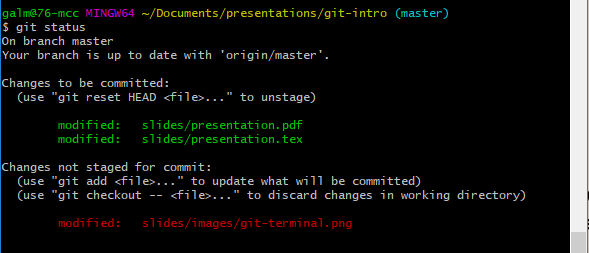
\includegraphics[width=0.8\linewidth]{images/git-status}
\end{figure}}<1>


\par\noindent\hrulefill\par

\textbf{What's changed?}

\code{git diff} lets us know the difference between the files we could stage, and the staged version of them

\only{\begin{figure}
	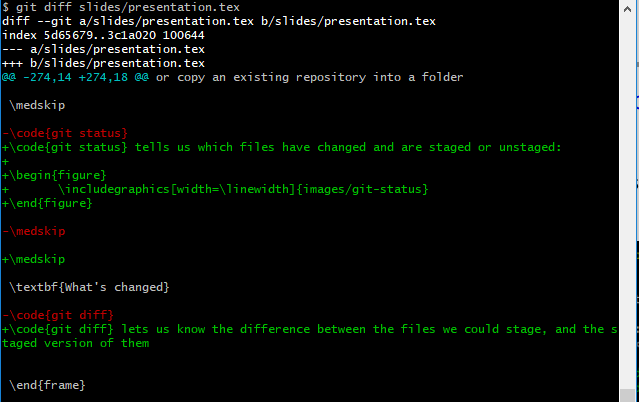
\includegraphics[width=0.8\linewidth]{images/git-diff}
\end{figure}}<2>

\only{\code{git diff} can also tell us about the difference between variously specified versions of files}<3>


\end{frame}
%--------------------------------------------------------------

% ==============================================================
\begin{frame}
	\frametitle{Navigating different versions}
	
	\code{git log} shows us a list of all the commits that have been made.
	
	\only{\begin{figure}
			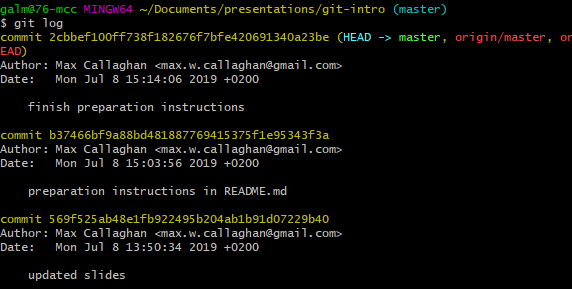
\includegraphics[width=0.8\linewidth]{images/git-log}
	\end{figure}}<1->

\par\noindent\hrulefill\par	

	\code{git checkout} takes you to another commit, or another branch of the repository
	
	\medskip
	
	\code{git checkout master} takes you back to the most recent commit on the master branch
	
	
\end{frame}
%--------------------------------------------------------------



% ==============================================================
%\begin{frame}
%\frametitle{Branches and merges}
%
%explain what branches are
%
%\code{git branch}
%
%\code{git merge \emph{branchname}}
%
%\code{git checkout}
%
%\end{frame}
%--------------------------------------------------------------

% ==============================================================
\begin{frame}
\frametitle{Interacting with remote repositories}

If you started a repository on your computer, you can associate it with an \textit{empty} GitHub repository. Follow the instructions on Github: 

\bigskip

\code{git remote add origin https://github.com/mcallaghan/blablabala.git}

\medskip

\code{git push -u origin master }

\bigskip

Now your local repository exists online, where it's current status and entire history is reflected.

\medskip

N.B. when dealing with the public domain, don't forget licenses (of your and other people's work).

\end{frame}
%--------------------------------------------------------------

\begin{frame}
	\frametitle{Interacting with remote repositories}
		
	\code{git pull} downloads all of the changes (commits) that are published in the remote version, and incorporates them (as long as they do not clash with your changes) into your local copy
	
	Merging is normally done automatically, but you may need to choose between different versions if they have both changed the same lines of code 
	
	\par\noindent\hrulefill\par		
	
	\code{git push} adds all of your committed changes to the remote version (as long as your version contains all of the changes in the remote - you need to \code{pull} first)
	
	\bigskip
	You can only \code{push} to repositories you have the correct permissions for, but you can make a \code{pull request} (a suggestion that your changes be merged into the master) for any repository. This allows changes to be reviewed and tested before incorporation.
	
\end{frame}
%--------------------------------------------------------------

% ==============================================================
\begin{frame}
\frametitle{Version control using GUIs}



\only<1>{You can also employ version control using a GUI such as Github Desktop, or within code editors e.g. Atom} 

\only<2-3>{\begin{figure}
		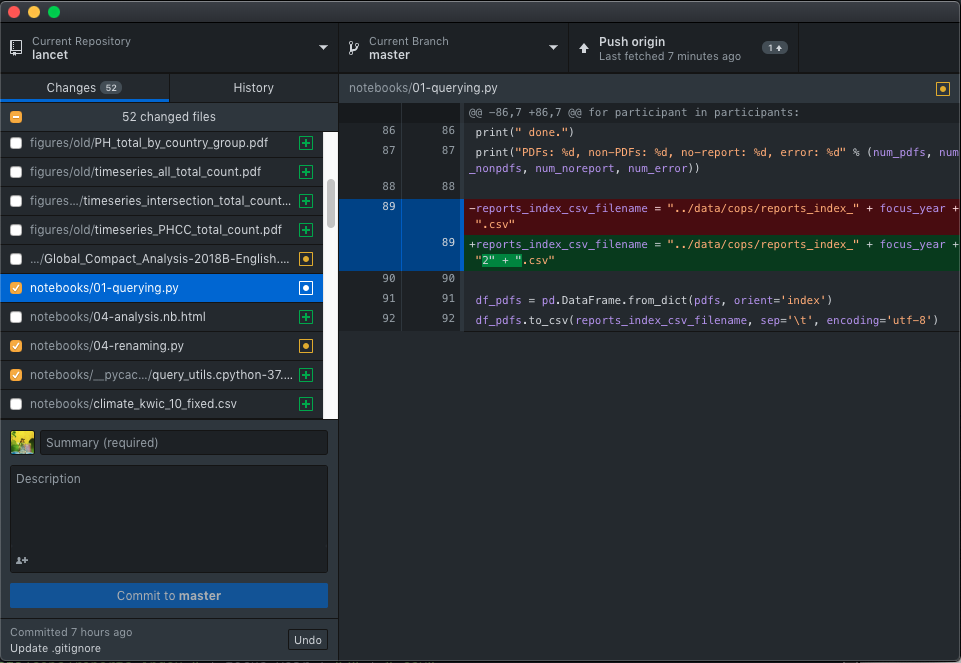
\includegraphics[width=0.8\linewidth]{images/gd-example}
\end{figure}}

\only<2>{The sidebar shows an equivalent of \code{git status} - you can see which files have been created or changed, and whether they have been added or staged for commit or not}

\only<3>{You can also see the changes you've made to files, similar to \code{git diff}}

\only<4>{\begin{figure}
		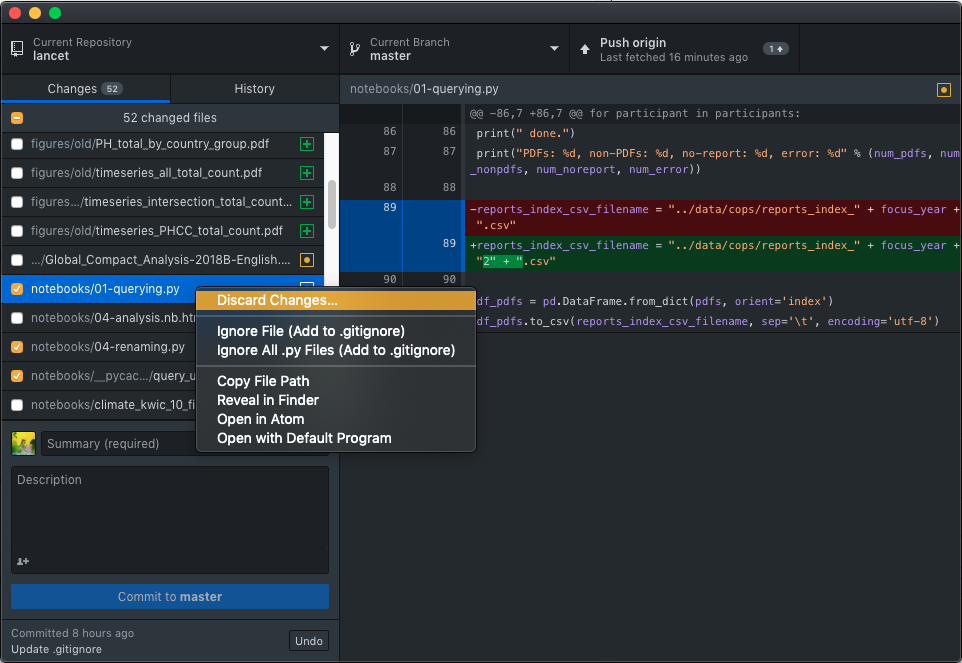
\includegraphics[width=0.8\linewidth]{images/gd-manage}
\end{figure}}

\only<4>{There are also options for you to stage or discard your changes, or add it to a list of files where changes are ignored}

\only<5>{\begin{figure}
		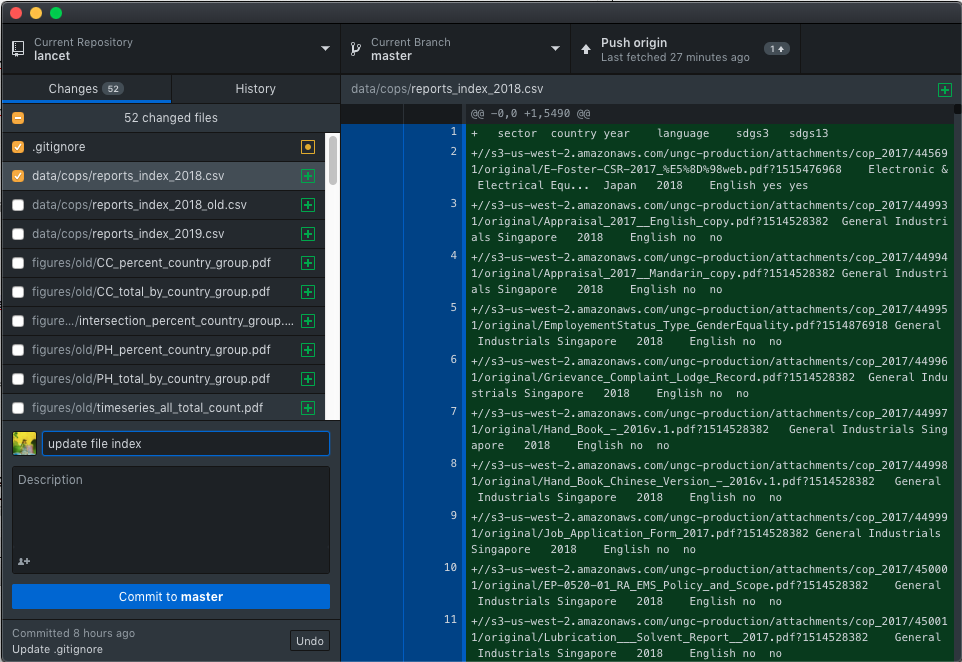
\includegraphics[width=0.8\linewidth]{images/gd-commit}
\end{figure}}

\only<5>{You can then review your changes and commit them, then push to the remote from the interface}

\end{frame}
%--------------------------------------------------------------

% ==============================================================
\begin{frame}
\frametitle{Further useful commands and tools}

\begin{itemize}
	\item \code{.gitignore} - A list of files, or patterns for git to ignore
	\item \href{https://guides.github.com/activities/citable-code/}{Zenodo} lets you get a citable DOI for your code/data
	\item \href{https://guides.github.com/features/pages/}{GitHub Pages} allows you to quickly turn your repository into a static website
	\item \href{https://github.com/mcc-apsis/git-intro/blame/master/slides/presentation.tex}{Blame} lets you trace, line by line, who contributed which parts of the code, and when
	
\end{itemize}

Github also has nice tools for making wikis and tracking issues, among other things, and can act as cloud storage, and a convenient way to browse the history of your project.

\bigskip

N.B. Sometimes Git is confusing! If you are about to do something you don't quite understand, you can copy the whole folder into another location for safe keeping. It's hard to lose data you have committed, but it is possible to lose changes you haven't committed.




\end{frame}
%--------------------------------------------------------------

% ==============================================================
\begin{frame}
\frametitle{}

{\huge
Questions?
}

\end{frame}
%--------------------------------------------------------------

% ==============================================================
\begin{frame}
\frametitle{Practice / task}

\begin{itemize}
\item Make a new project folder, and initialise a git repository with \code{git init}

\item Add a README.md file with some text in it.

\item Stage and commit your changes with \code{git add}, and \code{git commit}

\item Make a new empty repository on Github \url{https://github.com/new}

\item Follow the instructions to add this remote to your local repository with \code{git remote add origin [link]} and push your changes \code{git push -u origin master}

\item Find a partner, add each other as collaborators, edit each other's repositories, and push changes.


\end{itemize}




\end{frame}
%--------------------------------------------------------------


% ==============================================================
\begin{frame}
\frametitle{References}

\bibliographystyle{apalike}
\bibliography{bibliography}

\medskip
\par\noindent\hrulefill\par	
\medskip

Git is abundantly documented
\url{https://git-scm.com/doc}

\medskip Most ``How do I?'' git queries can be answered via a google search

\end{frame}
%--------------------------------------------------------------


\end{document}


